\chapter{Problem Analysis}
This chapter deals with the overall analysis of the problem itself. In the very beginning we present the definition of the problem. Every aspect of the problem is further discussed in detail along with a comparison of possible solutions. Moreover, the next section of the chapter describes data we work with and their alternatives. The final part of this chapter presents some of the important related works.

\section{Problem definition}

\section{Methods of generation}

\section{Data}
In previous part we talked about possible methods of generation. Another crucial aspect we need to discuss are data, which are a basic building block of our thesis. This part focuses on the analysis of the data we used in our thesis, but also on their alternatives. \\

In order to solve our task and train neural network we need to get dataset containing the X-rays images along with their textual descriptions and optionally some other attributes of the examined X-rays. Moreover, the fundamental feature we need is that the data must be in the Czech language.

\subsection{Existing datasets}
Medical environment provides a plenty of diverse potential problems, which can be researched. As already mentioned, in this thesis we focus specifically on the X-ray images. Because it is not so hard to detect fractures on the limbs, this area is not as interesting as others. One area that is rich in its diversity is the chest. As a result, this area is explored the most and therefore there exists multiple datasets with full textual mecidal reports. In the following section we describe some of them.

\subsubsection{Indiana University chest X-ray dataset}
Indiana University chest X-Ray dataset  has become a standard in the field of medical report generation, it was presented in the \citet{10.1093/jamia/ocv080} paper. This dataset is an open source collection of pairs of chest X-rays and their corresponding stuctured textual radiology reports, which is freely availble on the web\footnote[1]{\url{https://openi.nlm.nih.gov/faq\#collection}} without any additional requirements. We have a choice if we want to download just reports or images and in either PNG or DICOM format. The entire dataset consists of 7470 chest X-ray images that cover not only the frontal (PA\footnote[1]{Posterior-Anterior}) view, but also the lateral (side) one. These images corresponds to a total of 3995 patient's medical text reports.\\

Figure \hyperref[fig01:IUChestXRaySample]{1.1} shows an example from the Indiana University chest X-ray dataset. Each dataset pair is carefully de-identified in order to remove any personal information. The text of the report is structured in up to 5 sections. The most important sections are \textit{impression}, where the overall diagnosis is stated, \textit{findings} section describing the details of examination and \textit{tags} which are of two types - manual and automatic. Manual tags were annotated manually using MeSH\footnote[1]{\url{https://www.nlm.nih.gov/mesh/meshhome.html}} and RadLex\footnote[1]{\url{http://radlex.org/}} codes, automatic were encoded from the reports using the MTI indexer. The rest of the sections are \textit{indication} and \textit{comparison}.\\

The disadvantage of this dataset is that it is relatively small. On the other hand, it is a clean and manually checked dataset containing also additional information about images in a form of tags described above.

\begin{figure}[h]\centering
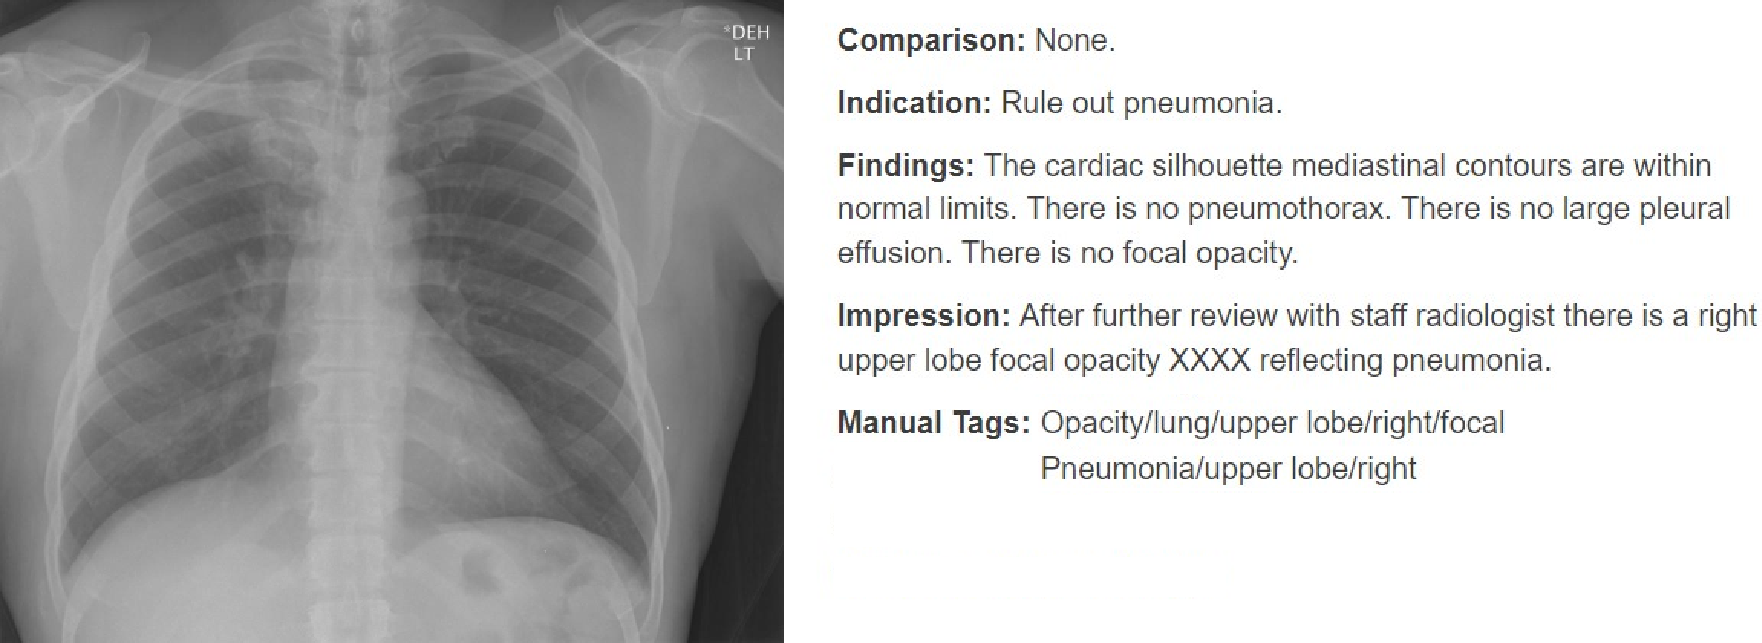
\includegraphics[width=145mm, height=53mm]{../img/IUChestXRaySample_CXR1728_IM-0479-1001}
\caption{Sample from the Indiana University Chest X-ray dataset.}
\label{fig01:IUChestXRaySample}
\end{figure}

\subsubsection{MIMIC-CXR}
MIMIC-CXR dataset description

\begin{figure}[h]\centering
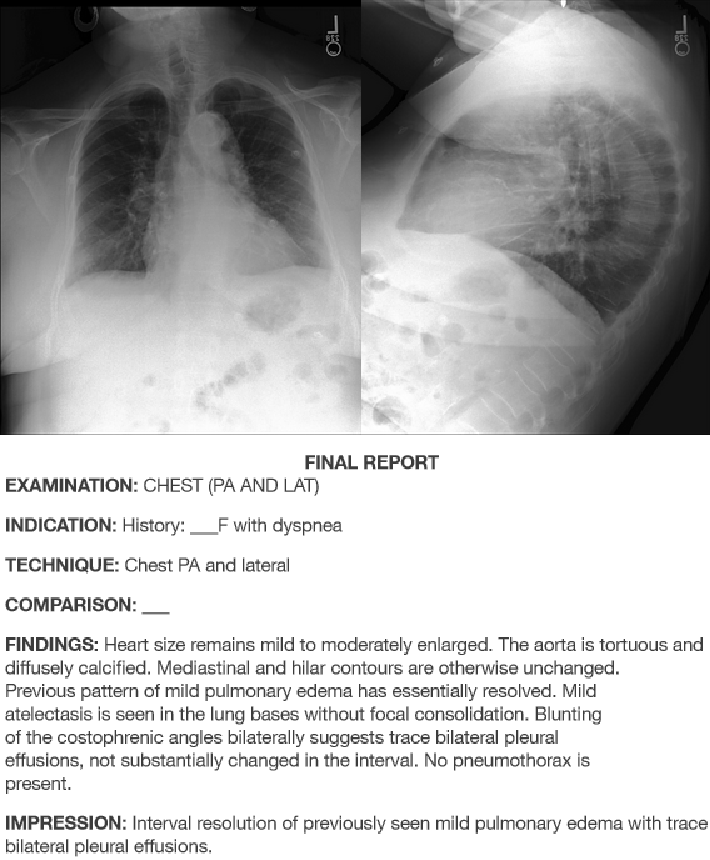
\includegraphics[width=135mm, height=163mm]{../img/mimic_s57861150}
\caption{Sample from the MIMIC-CXR dataset.}
\label{fig02:MimicCXRSample}
\end{figure}

\newpage

\subsection{Czech data}
All freely available datasets presented in the previous part have one common downside, namely they are not in the Czech language. As a part of elaboration of this thesis an intesive communication with real czech hospitals and other possible sources of real data took place. The goal of this communication was to create the very first open czech dataset of this kind. Processing of this kind of data would mean not only preparing the data into suitable format but also it would include proper anonymization of any personal information about the patients within the data. \\

However, inasmuch as the authentic patients data from hospitals are subject to strict privacy rules and we are not employees of any hospital, the institutions decided that they cannot provide the data in any way without the concious permission of patients given before the examination. With this result we need to find a different way how to obtain this much needed czech data.

\subsection{Translators}
In the previous sections we discovered that there is no dataset in the Czech language for our problem and there is no easy way how to get acces to the real data in order to build one. The only thing left is to create a new artificial dataset using an automatic translation. We will compare different freely accesible translators and choose the right one for our needs.

\subsubsection{DeepL}
At the moment, DeepL\footnote[1]{\url{https://www.deepl.com/translator}} translator provides the finest available translations beating even the ones from Google Translate. Moreover, it has freely usable web application and REST API. However, the main drawback of the DeepL translator is that its REST API is highly limited - only 500 000 characters per month can be translated for free. Furthermore, any translation above this limit is costly and thus this path is not appropriate for translating large textual datasets. One way to get around this problem is to use their internal REST API used specifically for the web application, which is free to use. We investigated and implemented this potential way in our thesis and further experimented how much it can be used, but unfortunately even this internal REST API is strictly limited for only tens of consecutive\footnote[2]{REST API calls are delayed from each other for some time, otherwise the service is blocked immediately} translations making it unusable for out needs.

\subsubsection{Google Translate}
Google~Translate\footnote[3]{\url{https://translate.google.com/}} has become already de facto standard in the world of machine translation and it is the most used freely accessible language translation service in the world. In terms of quality, the translations are still great although little bit worse than those from DeepL. The web application is free of any charge and anybody can use it as much as he needs. Nevertheless, just as in the case of DeepL, their REST API services are limited and translation of anything above that limit is expensively charged. For these reasons, as in the previous case, we must find another way.

\subsubsection{CUBBITT}
Machine~Translation\footnote[4]{\url{https://en.wikipedia.org/wiki/Machine\_translation}} is an extensive area of research, as a result of which there exist many other projects and academic papers nowadays. One of them is CUBBITT\footnote[5]{\url{https://lindat.mff.cuni.cz/services/translation/}} translator, which was developed at our faculty. The whole system is presented and described in detail in the \citet{biblio:PoToTransformingmachine2020} paper. \\

CUBBITT translator provides translations which are comparable to the ones from DeepL and Google Translate services. As other mentioned translators it provides an openly available web application for machine translation. Moreover and most importantly it provides REST API that is completely unlimited in text volume and free to use without any additional charges. These are the reasons why we will utilize CUBBITT in our thesis as a translator to create our artificial dataset.\\

On the other hand, CUBBITT has not support for auto-correcting input text compared to above mentioned services. Moreover, there are some patterns in the text which CUBBITT cannot translate at all or translates them incorrectly. These problems complicates our situation as the data from hospitals carry some natural noise in them. We face these complications in Chapter X.

\section{Language models}
\subsection{GPT2}

\section{Related work}
The last section of this chapter is dedicated to description and comparison to some of the related works that solves identical or similar problem as we do.









